\chapter{Simulation Studies}
\label{cha:simulation-result}

In this chapter, we lay out numerical results illustrating the computational and statistical efficiency of the algorithm proposed in Chapter~\ref{cha:methodology}. 

\iffalse
Throughout Chapter~\ref{cha:computational-acceleration}, we focus on the high-dimensional EM algorithm in large-Q regime, which is illustrated in Algorithm. We empirically study two cases using our algorithm: large-J regime and large-Q regime motivated this thesis. Before comparing the consistency rates and efficient, we provide the statement proved by Figure saying that the error between estimators given by base EM algorithm and Woodbury EM algorithm can be controlled near the machine error, which demonstrates that these two algorithms give the same estimation numerically.

Figure~\ref{fig:mode-equivalence} 

\begin{figure}[H]
    \centering
    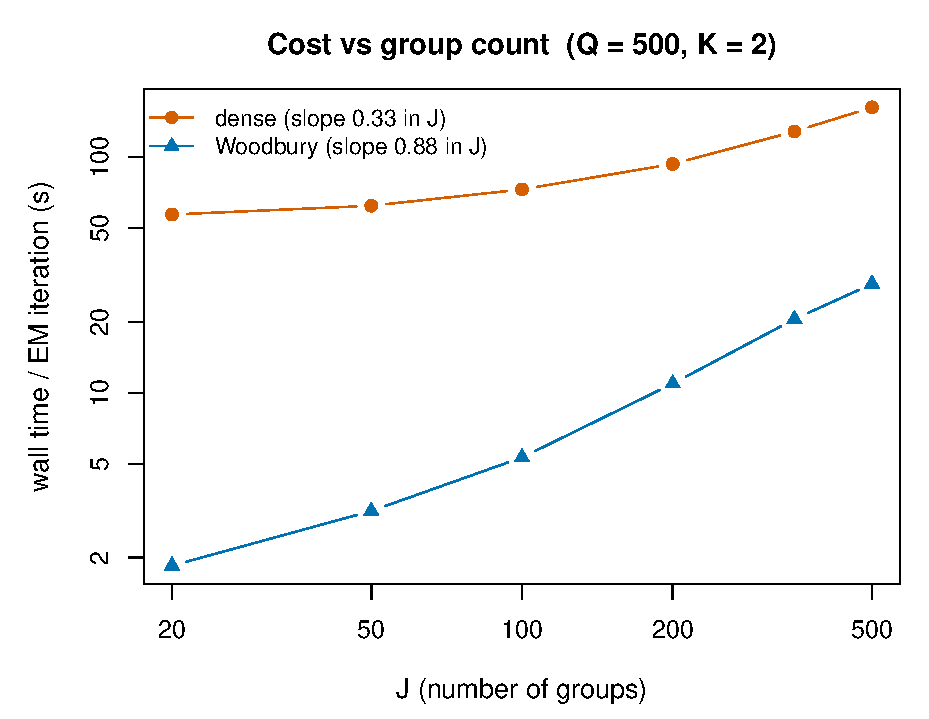
\includegraphics[width=0.8\textwidth]{figs/figJ_time.pdf}
    \caption{Time Cost Comparison.}
    \label{fig:cost-vs-group-count}
\end{figure}

The first result under large-J regime states that our Woodbury EM algorithm can reduce the cost of time when $J$ increasing, with large and fixed $Q$. Before the test on real-data, we do the simulation on generated dataset. 
\fi

\section{Evaluation Metrics}
\label{sec:sim-metrics}
The marginal likelihood depends on $B$ only through $\bm{\Sigma} = \mathbf{BB}^\top + \sigma^2 \mathbf{I}_Q$. This quantity is invariant under $\mathbf{B} \mapsto \mathbf{BQ}$ for any orthogonal $\mathbf{Q} \in O(K)$. The PLT-constraint fixes a unique representative $\mathbf{B}^{*}$ for the data-generating parameter, but this constraint is not enforced during estimation. Consequently $\hat{\mathbf{B}}$ can converge to a different rotation of the same column space as $\mathbf{B}^{*}$, and a direct entrywise comparison of $\hat{\mathbf{B}}$ to $\mathbf{B}^{*}$ is not meaningful.

We instead compare column spaces. Let
\[
\mathbf{P}_{\mathbf{B}} = \mathbf{B}(\mathbf{B}^\top \mathbf{B})^{-1}\mathbf{B}^\top
\]
denote the orthogonal projector onto $\mathrm{col}(\mathbf{B})$. We define the subspace distance
\[
d(\hat{\mathbf{B}}, \mathbf{B}^{*}) = \left\| \mathbf{P}_{\mathbf{B}} - \mathbf{P}_{\mathbf{B}^{*}}\right\|_F.
\]
This quantity is rotation-invariant and lies in $[0, \sqrt{2K}]$, with $0$ attained only when the two column spaces coincide. All references to \texttt{B\_dist} in the code correspond to this quantity.

Since $\sigma^2$ is a scalar, we report the signed relative error
\[
r(\hat\sigma^2, \sigma^{2\ast}) = \frac{\hat\sigma^2 - \sigma^{2\ast}}{\sigma^{2\ast}}.
\]
A negative value indicates shrinkage toward zero, which is the direction of the Heywood-case pathology. We keep the sign rather than reporting $|r|$, since the direction of the error is itself diagnostic.

\section{Simulated Data Generation}
\label{sec:sim-data}

\subsection{Generative Model}

Each simulated dataset is generated from the model of Chapter~\ref{cha:model-specification} directly to evaluate estimation error rather than model misspecification. Fixed $Q$ categories, $J$ groups, and $I_{j}$ observations per group, we draw the loading matrix $\mathbf{B} \in \mathbb{R}^{Q \times K}$ under the PLT identifiability constraint, which fixes the rotation and sign ambiguity in $\mathbf{B}$ and makes $\mathbf{B}^{*}$ be a single well-defined target rather than an equivalence class. For each group $j = 1, \dots, J$, we draw a $K$-dimensional factor score and an idiosyncratic term,
\[
\mathbf{f}_j \sim N(0, \mathbf{I}_K), \qquad \bm{\epsilon}_j \sim N(0, \sigma^2 \mathbf{I}_Q),
\]
and set the group-level random effect
\[
\bm{\lambda}_j = \mathbf{Bf}_j + \bm{\epsilon}_j \in \mathbb{R}^Q.
\]
Note that the latent factor $\mathbf{f}_j$ is never estimated. It is a device for generating $\bm{\lambda}_j$ with covariance $\bm{\Sigma} = \mathbf{BB}^\top + \sigma^2 \mathbf{I}_Q$ and keep consistent with the model's marginal specification. The linear predictor for the $i$-th observation in group $j$ is
\[
\bm{\eta}_{ij} = \bm{\mu} + \bm{\lambda}_j + \bm{v}_{ij}^\top \bm{\phi},
\]
which has been defined in~\ref{eq:linear-predictor}. The probability vector of categories is the softmax of $\bm{\eta_{ij}}$, defined together with observed count vector in~\ref{eq:conditional-pm}.

We vary $Q$, $J$, $I$ across scenarios holding $K$ known and fixed unless stated otherwise. The specific grids used in each experiment are given in the corresponding section. We do not fix a single canonical grid here since different questions require different ranges. 

\iffalse
Three regimes recur throughout this chapter and are worth naming in advance.
\begin{itemize}
\item \textbf{Fixed-$Q$, growing-$J$}: isolates how estimation error changes as the group-dimension grows, holding the amount of categories constant. 
\item \textbf{Fixed-$J$, growing-$Q$}: isolates how estimation error changes as the response dimension grows, holding the amount of group-level data constant. 
\item \textbf{Joint $(Q,J)$ growth}: grows both dimensions together following the rate implied by the growth condition $J \gg Q^c \log Q$.
\end{itemize}
\fi

\section{Convergence Diagnostics}
\label{sec:sim-convergence}

Our EM implementation originally stopped when the relative change in the marginal log-likelihood fell below a tolerance,

\begin{equation}
    \left| \frac{\ell(\hat{\bm{\theta}}_{n}) - \ell(\hat{\bm{\theta}}_{n-1})}{\ell(\hat{\bm{\theta}}_{n-1})} \right| < \mathrm{tol}.
\end{equation}

We found this criterion unreliable in the region of parameter space near the Heywood boundary, where $\sigma^2$ is small relative to the scale of $\mathbf{BB}^\top$. In a representative cell ($Q=400$, $J=10$), the likelihood-based criterion declared convergence at iteration 10, with $\hat\sigma_{10}^2 = 0.4463$. Running the same EM sequence to iteration 60 without stopping showed $\hat\sigma_{n}^2$ still declining until reaching $\hat\sigma_{60}^2=0.4051$. It's a further $9.2\%$ relative change after the criterion had already triggered. This is a known phenomenon in EM algorithms with high fractions of missing information. The log-likelihood surface can be extremely flat in a direction along which the parameter itself is still moving substantially. A likelihood-only stopping rule cannot detect this, since it only observes the flat direction.

To distinguish genuine convergence from this false-convergence pattern, we apply Aitken's acceleration to the trace of $\sigma^{2}$ itself instead of likelihood, which had been proposed by \citet{Louis1982}. Given three consecutive iterates $\sigma_{2(n-1)}, \sigma_{2(n)}, \sigma_{2(n+1)}$, the extrapolated limit is,
\begin{equation}
    \sigma^2_\infty \approx \sigma_{2(n+1)} - \frac{\left(\sigma_{2(n+1)} - \sigma_{2(n)}\right)^2}
{\sigma_{2(n+1)} - 2\sigma_{2(n)} + \sigma_{2(n-1)}}.
\end{equation}
For the same calibration cell, extrapolating from iterates 30, 40, 50, 60 predicted $\sigma^2_\infty \approx 0.4035$. A subsequent long run to $n=300$ with a strict tolerance ($\mathrm{tol}=10^{-8}$) confirmed $\hat\sigma^2$ stabilizing near $0.4024$ by $t \approx 220$, within $0.5\%$ of the extrapolated value. This validates Aitken extrapolation as a cheap diagnostic. It does not replace a long run, but it flags whether a short run's reported value should be trusted. We note that the estimation of loading matrix $\mathbf{B}$ does not share this behavior. Its convergence trace can be non-geometric and non-monotonic even after $\sigma^2$ has stabilized, so Aitken's acceleration is not applied to $\hat{\mathbf{B}}$ in this thesis. 

\section{exact\_Shat Switch}
\label{sec:sim-exact-shat}

\subsection{Motivation}

The Woodbury-accelerated E-step relies on a surrogate curvature derived from PME rather than the exact Hessian of the marginal likelihood. This surrogate makes the diagonal-plus-low-rank Woodbury structure available at all, since the exact Hessian does not share this structure in the same closed form and must be computed densely at cost $\mathcal{O}(Q^3)$. Before relying on the surrogate throughout the rest of this thesis, we need to know whether it introduces material estimation bias relative to the exact curvature. We denote the surrogate-curvature branch \texttt{exact\_Shat = FALSE} and the exact-curvature branch \texttt{exact\_Shat = TRUE}, and compare the two under otherwise identical settings with same seed, data, and initializations.

\subsection{Design \& Fundings}

In Chapter~\ref{cha:methodology}, we discuss the approximation of $\hat{\mathbf{S}}_{j}$ and its surrogate $\hat{\mathbf{S}}^{P}_{j}$ using PME. As shown in~\ref{prop:diff-s}, the exact curvature $\mathbf{H}_j(\boldsymbol\lambda)$ decomposes as $\mathbf{H}^P(\boldsymbol\lambda)$ plus a correction term involving only group $j$'s own data, $\{y_{ij}, \mathbf{p}_{ij}\}_{i \in \mathcal{I}_j}$. Since $\hat{\mathbf{S}}_j = \left(-\mathbf{H}_j(\hat{\boldsymbol\lambda}_j)\right)^{-1}$ and $\hat{\mathbf{S}}^P_j = \left(-\mathbf{H}^P(\hat{\boldsymbol\lambda}_j)\right)^{-1}$ are both obtained by inverting this per-group quantity at a fixed evaluation point $\hat{\boldsymbol\lambda}_j$, the discrepancy between them is itself a per-group object: it does not depend on $J$, the total number of groups, provided $\hat{\boldsymbol\lambda}_j$ is treated as given rather than re-estimated from the full $J$-group data. This is exactly the setting of our single-round design below, where each EM update starts from a fixed, externally chosen $\boldsymbol\lambda_j$ rather than one obtained by jointly fitting all $J$ groups; the conclusion does not extend, without further argument, to $\hat{\mathbf{S}}_j$ evaluated at the fully iterated EM's global estimate. This has two consequences for our design. First, it justifies holding $J$ fixed at a small value while varying $(Q, \sigma^2_{\mathrm{prior}})$ in this experiment, since the discrepancy under study is already determined at the single-group level. Second, we restrict each comparison to a single EM update, rather than iterating to convergence, so that the curvature discrepancy is isolated from the cross-round E/M feedback discussed in Chapter~\ref{ch:heywood}. We run one EM update from a fixed starting point under both branches and record the resulting parameter value. We repeat this for a range of $\sigma^2_{\mathrm{prior}}$ values away from and at the true generating value. We separately repeat the comparison as a function of $J$ at fixed $Q$, to empirically confirm the prediction of~\ref{prop:diff-s} that the TRUE-FALSE gap does not shrink as the amount of group-level data grows. [TODO: state the exact $(Q, J, \sigma^2_{\mathrm{prior}})$ grid used in the final run.]
\iffalse
\begin{table}[htbp]
\centering
% \input{tables/exact_shat_gap_by_Q.tex}
\caption{Gap between exact-curvature and surrogate-curvature single-round updates, as a function of $Q$ and $\sigma^2_{\mathrm{prior}}$.}
\label{tab:exact-shat-gap-Q}
\end{table}

The gap between the two branches grows with $\sigma^2_{\mathrm{prior}}$ and shrinks sharply with $Q$; at [XX] the gap is on the order of [YY\%], and by $Q = [ZZ]$ it is close to numerically negligible. This is consistent with the PME approximation improving as $Q$ grows, since the Poisson-conditioning argument underlying PME becomes tighter in that regime. At the reference point where $\sigma^2_{\mathrm{prior}}$ is set to the true generating value, the exact-curvature branch recovers only a small fraction of the single-round discrepancy between the surrogate estimate and the truth; this indicates that the surrogate curvature is not the dominant source of that discrepancy, and that whatever is driving it lies elsewhere in the estimation procedure, not in the PME approximation itself. [TODO: insert final recovered-fraction numbers once the multi-seed rerun is in.] The $J$-sweep comparison shows the two branches tracking each other closely across the full range tested, with no evidence that the gap reopens as $J$ grows.



\subsection{Conclusion}

Based on these results we treat \texttt{exact\_Shat = FALSE} as the default setting for the remainder of this thesis. The surrogate curvature introduces only a small, $Q$-shrinking discrepancy relative to the exact Hessian, while enabling the Woodbury acceleration documented in Chapter~\ref{ch:woodbury}; the exact branch is retained in the codebase for diagnostic use but is not needed for the estimation results reported below.


\section{Self-Recovery on Simulated Data}
\label{sec:sim-recovery}

\subsection{Design \& Fundings}

For each cell of a $(Q, J, N)$ grid we generate $R$ independent datasets from the model of Section~\ref{sec:sim-data}, fit the Woodbury-accelerated estimator to each, and compute the metrics of Section~\ref{sec:sim-metrics} against the known generating truth. Every run follows the dual convergence protocol of Section~\ref{sec:sim-convergence}. [TODO: state final $(Q,J,N,R)$ grid.]

\begin{table}[htbp]
\centering
% \input{tables/self_recovery_phi_mu.tex}
\caption{Bias and MSE of $\hat\phi$ and $\hat\mu$, reported separately for zero and nonzero coefficients, across the simulation grid.}
\label{tab:recovery-phi-mu}
\end{table}

\begin{table}[htbp]
\centering
% \input{tables/self_recovery_sigma2.tex}
\caption{Relative error of $\hat\sigma^2$, with Monte Carlo standard errors, across the simulation grid.}
\label{tab:recovery-sigma2}
\end{table}

\begin{table}[htbp]
\centering
% \input{tables/self_recovery_B.tex}
\caption{Subspace distance $d(\hat B, B^\ast)$, with Monte Carlo standard errors, across the simulation grid.}
\label{tab:recovery-B}
\end{table}

Recovery of $\phi$ is [accurate/biased] for nonzero coefficients across the grid, with the expected lasso shrinkage bias toward zero; recovery of the zero coefficients shows [TODO: describe selection behavior once the table is in]. The relative error of $\hat\sigma^2$ is systematically negative across most of the grid, consistent with the shrinkage pathology documented in Chapter~\ref{ch:heywood}; we do not attempt to correct for this here, and refer the reader to that chapter for the mechanism and candidate fixes. The magnitude of this negative bias is largest when $J$ is small relative to $Q$ and shrinks as $J$ grows, consistent with the classical degrees-of-freedom story for variance-component estimation. Subspace recovery of $B$ improves with $J$ at every $Q$ tested, though we note in Chapter~\ref{ch:asymptotics} that this improvement is not always monotone over the full EM trajectory, and the numbers reported here reflect estimates at the converged iteration count under the protocol of Section~\ref{sec:sim-convergence}, not at an arbitrary early stopping point.

\subsection{Known Limitation}
\label{sec:heywood-limitation}

As noted above, $\hat\sigma^2$ is biased downward in the regime where $\sigma^2$ is small relative to the scale of $BB^\top$, a pathology we refer to throughout this thesis as the Heywood case. This is a genuine limitation of the current estimator and is treated as a separate problem in Chapter~\ref{ch:heywood}, rather than as a defect specific to the Woodbury acceleration; the same pathology is present, to varying degrees, in every package compared against in Section~\ref{sec:sim-comparison} below.


\section{Comparison Against Existing Packages}
\label{sec:sim-comparison}

\subsection{Design \& Fundings}

We fit the same simulated datasets under three existing packages, chosen to isolate different components of the FA-DMR model. \texttt{glmnet} provides a lasso-penalized comparison for $\hat\phi$ alone, with no random-effect structure. \texttt{glmmTMB} provides a comparison for the random-effect variance component under a standard GLMM, without the factor-analytic structure on $\alpha_j$. \texttt{gllvm} provides the closest comparison overall, since it fits the same generalized-linear-latent-variable family under a Laplace approximation option, and is therefore treated as the primary benchmark rather than a secondary check. For each package we record both estimation accuracy, using the metrics of Section~\ref{sec:sim-metrics} restricted to the components that package estimates, and wall-clock runtime.

\begin{table}[htbp]
\centering
% \input{tables/package_comparison_accuracy.tex}
\caption{Estimation accuracy of the Woodbury estimator against glmnet, glmmTMB, and gllvm, restricted to the parameter components each package estimates.}
\label{tab:comparison-accuracy}
\end{table}

\begin{table}[htbp]
\centering
% \input{tables/package_comparison_runtime.tex}
\caption{Wall-clock runtime comparison across packages, at matched $(Q,J,N)$.}
\label{tab:comparison-runtime}
\end{table}

The Woodbury estimator matches \texttt{glmnet} and \texttt{glmmTMB} on the components those packages estimate, while running substantially faster, consistent with the acceleration results of Chapter~\ref{ch:woodbury}. Against \texttt{gllvm}, the fairer comparison given the shared model family, the Woodbury estimator is currently [somewhat behind / comparable] on estimation accuracy; [TODO: state final direction and magnitude once the rerun is in, and note whether this gap is concentrated in the Heywood regime or present throughout the grid]. We treat \texttt{gllvm}'s relative accuracy advantage as a target for the refinements discussed in Chapter~\ref{ch:heywood}, rather than as evidence against the Woodbury architecture itself, since the runtime advantage documented here is retained regardless.

\subsection{Discussion}

The comparison is not fully symmetric: \texttt{glmnet} and \texttt{glmmTMB} do not model the factor structure on $\alpha_j$ at all, so their accuracy numbers reflect an easier estimation problem restricted to a subset of parameters, not a head-to-head comparison on the full model. \texttt{gllvm} is the only package tested that estimates a comparable factor-analytic structure, and is therefore the benchmark we weight most heavily in interpreting these results. [TODO: add any covariate-recovery comparison if run.]
\fi


